\documentclass[11pt]{article}

\usepackage[T1]{fontenc}
\usepackage[utf8]{inputenc}
\usepackage{lmodern}
\usepackage[a4paper,margin=1in]{geometry}
\usepackage{amsmath,amssymb,amsthm,mathtools}
\usepackage{float}
\usepackage{enumitem}
\usepackage{booktabs}
\usepackage{xcolor}
\usepackage{listings}
\usepackage{tikz}
\usepackage{hyperref}
\usetikzlibrary{arrows.meta,positioning,calc,fit,backgrounds,shapes.geometric}

\hypersetup{
    colorlinks=true,
    linkcolor=blue!70!black,
    citecolor=blue!70!black,
    urlcolor=blue!70!black
}

% ── Theorem environments ──────────────────────────────────────────────────────
\newtheorem{theorem}{Theorem}[section]
\newtheorem{proposition}[theorem]{Proposition}
\newtheorem{lemma}[theorem]{Lemma}
\newtheorem{corollary}[theorem]{Corollary}
\theoremstyle{definition}
\newtheorem{definition}[theorem]{Definition}
\newtheorem{example}[theorem]{Example}
\theoremstyle{remark}
\newtheorem{remark}[theorem]{Remark}

% ── Geometry / coloring macros ────────────────────────────────────────────────
\newcommand{\dist}{\operatorname{dist}}
\newcommand{\UDG}{\operatorname{UDG}}
\newcommand{\MWIS}{\mathrm{MWIS}}
\newcommand{\MIS}{\mathrm{MIS}}
\newcommand{\Efalse}{E_{\mathrm{false}}}
\newcommand{\Etrue}{E_{\mathrm{true}}}
\newcommand{\chihat}{\widehat{\chi}}
\newcommand{\R}{\mathbb{R}}
\newcommand{\N}{\mathbb{N}}
\newcommand{\indep}{\alpha}
\newcommand{\Gen}{\mathsf{Gen}}

% ── Type-system macros (problem-types / certified reductions) ─────────────────
\newcommand{\Col}{\mathsf{Col}}
\newcommand{\ISt}{\mathsf{IS}}
\newcommand{\WIS}{\mathsf{WIS}}
\newcommand{\tUDG}{\mathsf{UDG}}
\newcommand{\tUDGa}{\widetilde{\mathsf{UDG}}}
\newcommand{\Dev}{\mathsf{Dev}}
\newcommand{\Sol}{\mathrm{Sol}}
\newcommand{\Nmax}{N_{\max}}
\newcommand{\safe}{\textsf{safe}}
\newcommand{\asafe}[1]{\textsf{asafe}(#1)}
\newcommand{\realizes}{\mathsf{realizes}}
\newcommand{\falsep}{\mathsf{false}}
\newcommand{\miss}{\mathsf{miss}}
\newcommand{\totopt}{\mathsf{tot\text{-}opt}}
\newcommand{\rn}[1]{\textsc{\footnotesize #1}}
\newcommand{\irule}[2]{\ensuremath{\dfrac{\;#1\;}{\;#2\;}}}
\newcommand{\redto}[1]{\mathrel{\overset{\textstyle #1}{\rightsquigarrow}}}
\newcommand{\redtos}[2]{\mathrel{\overset{\textstyle #1}{\underset{#2}{\rightsquigarrow}}}}
\newcommand{\idearemark}[1]{%
  \par\smallskip\noindent
  \fcolorbox{black}{yellow!12}{%
    \parbox{\dimexpr\linewidth-2\fboxsep-2\fboxrule\relax}{\textbf{Key point.}\ #1}}%
  \par\smallskip}

% ── Listings style for the surface language ────────────────────────────────────
\lstdefinestyle{lang}{
  basicstyle=\ttfamily\small,
  columns=fullflexible,
  keepspaces=true,
  frame=single,
  showstringspaces=false,
  breaklines=true,
  keywordstyle=\bfseries\color{blue!55!black},
  commentstyle=\itshape\color{green!40!black},
  morekeywords={graph,palette,colors,size,udg,radius,vertices,edges,restrictions,
    transform,toUDG,exact,preserve,compose,encodeColoring,superUDG,colorChoice,
    gadgetize,layout,emit,color,using,subjectTo,via,apply,to,chromaticNumber,
    kColorable,chromatic,bipartite,let,where,instance,compute,precolor,allow,
    forbid,sameColor,differentColor,useAtMost,useExactly,distinctOn,keep,drop,
    trackOrigin,safe,asafe,data,type},
  morecomment=[l]{--}
}
\lstdefinestyle{plain}{
  basicstyle=\ttfamily\small,
  columns=fullflexible,
  keepspaces=true,
  frame=single,
  showstringspaces=false,
  breaklines=true
}

% ── Lightweight algorithm float (no algorithmicx dependency) ───────────────────
\newfloat{algorithm}{htbp}{loa}
\floatname{algorithm}{Algorithm}
\newcommand{\Comment}[1]{\hfill\textit{\footnotesize\textcolor{gray}{// #1}}}

% ─────────────────────────────────────────────────────────────────────────────
\title{%
  \textbf{Certified Compilation of Graph Coloring to Neutral-Atom Hardware}\\[0.45em]
  \large An Exact Gadgetized Reduction, a Heuristic Layout Optimizer,\\
  and a Type-and-Effect Discipline for the Pipeline}
\author{Research Draft}
\date{\today}

\begin{document}
\maketitle

\begin{abstract}
Neutral-atom quantum processors solve a single native problem: maximum-weight
independent set (MWIS) on a unit-disk graph (UDG), realized physically by the
Rydberg blockade. They do \emph{not} color graphs. We present a compilation pipeline
that takes an arbitrary finite graph-coloring instance and produces a
hardware-executable UDG--MWIS instance whose ground state decodes back to a proper
coloring of the original graph, together with a small typed language that makes the
pipeline's correctness static. The pipeline has two layers with a clean separation
of concerns. The \emph{primary path} is an exact, polynomial-time two-stage
reduction: a textbook reduction of $k$-colorability to maximum independent set on an
auxiliary graph $G'$ of size $nk$, followed by a gadgetized embedding of $G'$ into a
weighted UDG using copy and crossing gadgets in the style of Nguyen et al.
Correctness here is a once-proved meta-theorem, not a per-instance gamble: there is
no chromatic-number inflation and the decoder is an exact inverse. The genuine
engineering uncertainty therefore moves out of correctness and into \emph{geometry}:
atom count, array area, crossing number, and analog-solve quality. The
\emph{secondary path} is a suite of seven polynomial-time geometric heuristics; we
prove an impossibility result that disqualifies them as a stand-alone coloring
mechanism for general graphs and repurpose them as the \emph{layout optimizer} that
places and compacts the gadgetized instance under hardware constraints. We then
introduce a Haskell-flavored surface language and a \emph{type-and-effect discipline}
in which every compilation stage is typed as an answer-preserving morphism carrying
an executable decoder, and same-vertex transforms carry a \emph{safety effect}
bounding chromatic inflation; a single composition rule yields end-to-end soundness.
The type discipline situates the work in the line of type-and-effect systems for
behavioral policies developed by Gian-Luigi Ferrari and collaborators, to whom this
paper is dedicated.
\end{abstract}

\paragraph{Keywords.} graph coloring, unit-disk graphs, maximum independent set,
Rydberg blockade, neutral-atom computing, gadget reductions, certified compilation,
type-and-effect systems, QuEra, Bloqade.

\tableofcontents
\newpage

% =============================================================================
\section{Introduction}
\label{sec:intro}
% =============================================================================

Graph coloring is a canonical NP-complete problem~\cite{Karp1972,GareyJohnson1979}
with broad practical reach, from register allocation and scheduling to frequency
assignment. A recent and physically distinctive way to attack such combinatorial
problems is the neutral-atom quantum platform, in which individually trapped atoms
are excited to Rydberg states and interact through the \emph{Rydberg
blockade}~\cite{Saffman2010,Henriet2021,Scholl2022}. The decisive feature of this
platform is geometric: two atoms within a blockade radius $r$ cannot both be excited,
so the set of simultaneously excited atoms is precisely an \emph{independent set} of
the unit-disk graph (UDG) induced by atom positions. The device's analog ground state
therefore encodes a \emph{maximum-weight independent set} (MWIS) of that
UDG~\cite{Pichler2018,Ebadi2022}.

This single fact frames the entire compilation problem and is the pivot of this
paper:

\begin{quote}
\itshape
The hardware solves MWIS on a unit-disk graph. It does not color. Any pipeline that
compiles coloring to this hardware must \emph{reduce} coloring to UDG--MWIS, not
merely \emph{embed} the input graph geometrically.
\end{quote}

\subsection{Two tempting designs, and why one is correct}

There are two natural strategies for getting an arbitrary coloring instance onto this
hardware.

\paragraph{Design A --- geometric supergraph embedding.} Place the original vertices
in $\R^2$ and choose a radius $r$ so that the induced UDG $H$ is a \emph{supergraph}
of the input $G$, i.e.\ $E(G)\subseteq E(H)$. Then any proper coloring of $H$
restricts to a proper coloring of $G$. This is attractive because the supergraph
relation is trivially achievable and gives a one-line decoder.
Section~\ref{sec:heuristics} develops the seven heuristics that make $H$ as good as
possible. However, Design A has two structural defects. First, we prove
(Theorem~\ref{thm:impossibility}) that a same-vertex UDG supergraph \emph{cannot}
bound chromatic-number inflation in general: the star $K_{1,n}$ has $\chi = 2$ but
forces $\chi(H)\ge\lceil n/5\rceil\to\infty$ in any UDG supergraph. Second, and
independently, even a perfect $H$ is not executable, because the device cannot color
$H$; coloring a UDG on an MWIS machine requires iterated independent-set extraction,
which is itself heuristic. Design A is thus heuristic twice and unbounded once.

\paragraph{Design B --- exact gadgetized reduction.} Reduce $k$-colorability of $G$ to
a \emph{single} MWIS instance, then embed that instance into a weighted UDG the
hardware can run. This is the standard reduction route, and it composes two exact,
polynomial-time steps (Section~\ref{sec:gadget}): the classical
colorability$\to$independent-set reduction, and the Rydberg gadgetization of an
arbitrary graph into a UDG via copy/crossing gadgets~\cite{Nguyen2023}. Here
correctness is a once-proved meta-theorem with no inflation and an exact inverse
decoder. The remaining uncertainty is not about \emph{whether} the answer is correct
but about \emph{whether it fits the device and whether the analog dynamics finds the
ground state} --- both geometric/physical questions.

We adopt Design B as the primary path and retain Design A's heuristics in a strictly
subordinate, and now sound, role: the \emph{layout optimizer} that realizes the
gadgetized instance under hardware spacing while minimizing atom count, area, and
crossings. Because the gadget structure is fixed and exact, the heuristics can no
longer affect correctness --- only feasibility and solve quality. This relocation is
the central design decision of the paper.

\subsection{From a pipeline to a typed language}

Once correctness lives entirely in a fixed chain of exact reductions, it becomes
natural to make that chain \emph{statically checkable}. The second half of the paper
introduces a small surface language --- Haskell-flavored, but deliberately restricted
--- whose types are not ordinary data types but \emph{problem-types} (``a $k$-coloring
instance on $n$ vertices,'' ``a weighted-IS instance with offset $C$,'' ``a unit-disk
instance that fits the device''), and whose arrows are \emph{certified reductions}
carrying executable decoders. The type system makes provenance, stage ordering, the
device budget, and chromatic-safety part of typing, so that a well-typed program is a
pipeline whose measured bitstring is guaranteed to decode to a correct coloring. The
chromatic-safety annotation is a \emph{type-and-effect}~\cite{LucassenGifford1988} in
the lineage developed by Gian-Luigi Ferrari and collaborators
\cite{BartolettiDeganoFerrariZunino2009,DeganoFerrariGalletta2016}, to whose work
this paper is dedicated.

\subsection{Contributions}

\begin{enumerate}[label=(\arabic*),leftmargin=2.2em]
  \item A clean statement of the compilation problem that takes the hardware's native
        primitive (UDG--MWIS) as the target, and a two-layer pipeline that separates
        exact correctness from heuristic geometry
        (Sections~\ref{sec:problem}--\ref{sec:gadget}).
  \item The exact primary reduction: colorability$\to$MIS with a self-contained
        correctness proof and size $nk$ (Theorem~\ref{thm:col2is}), composed with
        Rydberg UDG gadgetization (Theorem~\ref{thm:gadget}) to give an end-to-end
        exactness and decoding meta-theorem (Theorem~\ref{thm:endtoend}), together
        with $O((nk)^2)$ atom-count and feasibility bounds (Section~\ref{sec:size}).
  \item An impossibility result (Theorem~\ref{thm:impossibility}) that rigorously
        explains why the geometric-supergraph approach cannot be the correctness
        mechanism, justifying its demotion; and seven polynomial-time geometric
        heuristics, corrected and re-targeted as a hardware-aware \emph{layout
        optimizer} with termination guarantees (Section~\ref{sec:heuristics}).
  \item An integrated pipeline with worked examples, tables, figures, and a full
        complexity accounting (Sections~\ref{sec:pipeline}--\ref{sec:complexity}).
  \item A Haskell-flavored surface language (Section~\ref{sec:language}) and a
        type-and-effect discipline (Section~\ref{sec:types}) that turns the reduction
        theorems into typing rules, with a pipeline-soundness theorem and a
        safety-effect monoid that answers the open question of whether transform order
        affects safety.
\end{enumerate}

% =============================================================================
\section{Literature Review}
\label{sec:related}
% =============================================================================

\paragraph{Graph coloring and its complexity.} Deciding $k$-colorability for
$k\ge 3$ is NP-complete~\cite{Karp1972,GareyJohnson1979}, and the chromatic number is
hard even to approximate. Practical colorings are produced by greedy orderings such as
largest-first~\cite{Welsh1967} and by the saturation-degree heuristic
DSATUR~\cite{Brelaz1979}; the clique number gives the basic lower bound
$\omega(G)\le\chi(G)$~\cite{West2001}. We use DSATUR only as an auxiliary
\emph{witness} generator in the secondary path, never on the exact path.

\paragraph{Unit-disk graphs.} UDGs are the intersection graphs of unit disks in the
plane~\cite{Clark1990UDG}. Recognition --- deciding whether a given abstract graph is
a UDG --- is NP-hard~\cite{Breu1998,Jungck2021}, which is precisely why we never
attempt exact realization of the input graph. UDGs enjoy strong geometric locality:
every clique lies inside a disk of radius $r$, and the packing of points in such a
disk is bounded~\cite{Heppes2003}, a fact we use both for the impossibility result and
for clique control. The exactly-realizable one-dimensional families are the
unit/proper-interval graphs~\cite{Roberts1969,Golumbic1980}.

\paragraph{Rydberg MWIS and gadgetized reductions.} The identification of the Rydberg
blockade ground state with MWIS on a UDG is due to Pichler et al.~\cite{Pichler2018}
and was demonstrated at scale on hundreds of atoms by Ebadi et al.~\cite{Ebadi2022}.
Because native UDGs are geometrically restricted, Nguyen et al.~\cite{Nguyen2023}
introduced copy and crossing gadgets that encode MWIS on an \emph{arbitrary} graph as
MWIS on a weighted UDG laid out on a grid, with a known value offset and a structural
decoder. Our primary path is exactly the composition of the classical
colorability$\to$MIS reduction with this gadgetization; the hardware target is QuEra's
neutral-atom machine~\cite{Wurtz2023,Graham2022}, programmed through the Bloqade
simulation stack. Variational and analog quantum optimization more broadly is surveyed
in~\cite{Cerezo2021,Preskill2018}.

\paragraph{Spectral and force-directed layout.} Our layout optimizer draws on
classical embedding machinery: the graph Laplacian and its
eigenvectors~\cite{Chung1997,Fiedler1973}, Laplacian eigenmaps~\cite{Belkin2003},
force-directed drawing~\cite{Fruchterman1991}, multidimensional
scaling~\cite{Kruskal1964}, and gradient-based
optimization~\cite{Nesterov2004,Boyd2004}, with Pareto selection over the
radius~\cite{Miettinen2014}. These are standard tools; our contribution is not the
tools but their re-targeting to a \emph{correctness-neutral} role behind an exact
reduction.

\paragraph{Type-and-effect disciplines and certified transformation.} Our type system
(Section~\ref{sec:types}) is a \emph{type-and-effect} system in the lineage initiated
by Lucassen and Gifford~\cite{LucassenGifford1988} and developed extensively by
Gian-Luigi Ferrari and his collaborators, who used types and effects to make security
and resource-usage policies static and statically
enforceable~\cite{BartolettiDeganoFerrariZunino2009,DeganoFerrariGalletta2016,BodeiDeganoFerrari1998}.
In that tradition an \emph{effect} soundly over-approximates a computation's runtime
behavior so that a policy can be checked \emph{before} execution; the slogan that base
types certify well-formedness while effects certify a behavioral policy is directly
inherited from this line of work. We adopt exactly this idea for a different invariant
--- \emph{chromatic safety} --- annotating each same-vertex transform with a safety
effect drawn from a monoid ($\safe$ / $\asafe{c}$) that bounds chromatic inflation, so
that the order-sensitivity of safety becomes a checkable property rather than a
conjecture (Section~\ref{sec:safety}). It is a pleasure to dedicate this connection,
and the paper, to Gian-Luigi Ferrari, in whose honor this special issue appears: the
certified-reduction calculus developed here is, in spirit, a behavioral
type-and-effect system, transplanted from the world of secure service composition to
the world of quantum-hardware compilation.

% =============================================================================
\section{Problem Formulation}
\label{sec:problem}
% =============================================================================

We consider finite simple undirected graphs $G=(V,E)$ with $n=|V|$, $m=|E|$.

\begin{definition}[Proper $k$-coloring; chromatic number]
A proper $k$-coloring is a map $c:V\to\{1,\dots,k\}$ with $c(u)\ne c(v)$ for every
$\{u,v\}\in E$. The chromatic number $\chi(G)$ is the least $k$ admitting one.
\end{definition}

\begin{definition}[Unit-disk graph]
Given a placement $p:V\to\R^2$ and radius $r>0$, the induced UDG $\UDG(p,r)$ has an
edge $\{u,v\}$ iff $\|p(u)-p(v)\|_2\le r$. A weighted UDG additionally assigns a
weight $w:V\to\R_{>0}$.
\end{definition}

\begin{definition}[Independent set; MWIS]
An independent set of $H$ is a vertex set with no internal edge. For weights $w$, the
maximum-weight independent set value is
$\MWIS(H,w)=\max\{\sum_{v\in S}w(v):S\text{ independent}\}$. For unit weights this is
the independence number $\indep(H)$.
\end{definition}

\paragraph{Hardware primitive.} A neutral-atom array with atoms at positions $p(v)$
and blockade radius $r$ realizes $\UDG(p,r)$; under appropriate driving its many-body
ground state encodes $\MWIS(\UDG(p,r),w)$, where $w$ is set by local
detunings~\cite{Pichler2018,Ebadi2022}. The device constraints are a minimum atom
spacing $d_{\min}$, a maximum blockade radius $r_{\max}$, a finite array area
$A_{\max}$, and a maximum atom count $N_{\max}$~\cite{Wurtz2023}.

\paragraph{The compilation problem.} Given $(G,k)$ and the device parameters, produce
(i) a weighted UDG instance $A$ realizable on the array, and (ii) a decoder $\delta$,
such that from any MWIS of $A$ measured by the device, $\delta$ recovers a proper
$k$-coloring of $G$ whenever one exists, and otherwise soundly reports
non-$k$-colorability. The compilation itself must be polynomial time; only the analog
solve is left to the physics.

\paragraph{The two-layer pipeline.} Figure~\ref{fig:overview} shows the design. The
primary (exact) path reduces coloring to an \emph{abstract} weighted UDG--MWIS
instance and decodes the measured independent set back to a coloring. The secondary
(heuristic) path is the geometric engine that turns the abstract gadget instance into
concrete atom coordinates obeying the hardware constraints, and is also available as a
stand-alone --- but only chromatic-non-decreasing --- coloring backend for comparison.

\begin{figure}[h]
\centering
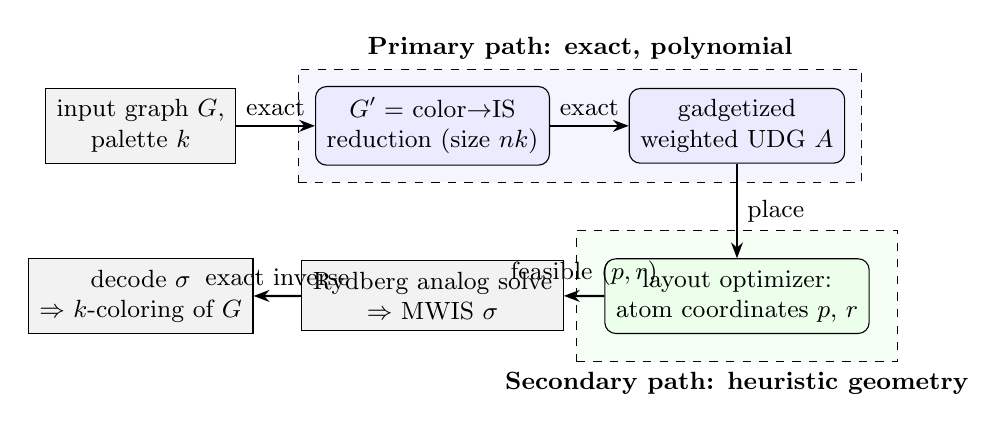
\begin{tikzpicture}[
  font=\small,
  node distance=8mm,
  exact/.style={rectangle,draw,rounded corners,fill=blue!8,minimum height=8mm,align=center,inner sep=4pt},
  heur/.style={rectangle,draw,rounded corners,fill=green!8,minimum height=8mm,align=center,inner sep=4pt},
  io/.style={rectangle,draw,fill=gray!10,minimum height=8mm,align=center,inner sep=4pt},
  ar/.style={-{Stealth[length=2mm]},thick}
]
\node[io] (G) {input graph $G$,\\ palette $k$};
\node[exact,right=10mm of G] (Gp) {$G'=$ color$\to$IS\\ reduction (size $nk$)};
\node[exact,right=10mm of Gp] (A) {gadgetized\\ weighted UDG $A$};
\node[heur,below=12mm of A] (layout) {layout optimizer:\\ atom coordinates $p$, $r$};
\node[io,below=12mm of Gp] (solve) {Rydberg analog solve\\ $\Rightarrow$ MWIS $\sigma$};
\node[io,below=12mm of G] (dec) {decode $\sigma$\\ $\Rightarrow$ $k$-coloring of $G$};

\draw[ar] (G) -- node[above]{exact} (Gp);
\draw[ar] (Gp) -- node[above]{exact} (A);
\draw[ar] (A) -- node[right]{place} (layout);
\draw[ar] (layout) -- node[above]{feasible $(p,r)$} (solve);
\draw[ar] (solve) -- node[above]{exact inverse} (dec);

\begin{scope}[on background layer]
  \node[draw,dashed,fill=blue!4,fit=(Gp)(A),inner sep=6pt,label=above:{\textbf{Primary path: exact, polynomial}}] {};
  \node[draw,dashed,fill=green!4,fit=(layout),inner sep=10pt,label=below:{\textbf{Secondary path: heuristic geometry}}] {};
\end{scope}
\end{tikzpicture}
\caption{The two-layer pipeline. Correctness lives entirely in the blue (exact) path;
the green (heuristic) path determines only hardware feasibility and analog-solve
quality.}
\label{fig:overview}
\end{figure}

% =============================================================================
\section{The Transformation, Step by Step}
\label{sec:gadget}
% =============================================================================

The primary path is the composition of two exact reductions:
\[
  \underbrace{G,k}_{\text{coloring}}
  \;\xrightarrow{\;\text{Stage 1}\;}\;
  \underbrace{G'}_{\text{MIS instance, size }nk}
  \;\xrightarrow{\;\text{Stage 2}\;}\;
  \underbrace{A=(\,p,r,w\,)}_{\text{weighted UDG}}
  \;\xrightarrow{\;\text{solve}\;}\;
  \sigma
  \;\xrightarrow{\;\text{decode}\;}\;
  \text{coloring of }G.
\]

\subsection{Stage 1: Colorability $\to$ Independent Set}
\label{sec:col2is}

\begin{definition}[Color-choice graph]
\label{def:choice}
Given $G=(V,E)$ and palette size $k$, the \emph{color-choice graph} $G'=(V',E')$ has
vertex set $V'=V\times\{1,\dots,k\}$, and edge set
$E'=E'_{\mathrm{choice}}\cup E'_{\mathrm{conflict}}$ where
\begin{align*}
  E'_{\mathrm{choice}}   &= \bigl\{\{(v,i),(v,j)\} : v\in V,\ 1\le i<j\le k\bigr\},
   &&\text{(a $k$-clique per vertex)}\\
  E'_{\mathrm{conflict}} &= \bigl\{\{(u,i),(v,i)\} : \{u,v\}\in E,\ 1\le i\le k\bigr\}.
   &&\text{(same-color conflicts)}
\end{align*}
All vertices carry unit weight. Then $|V'|=nk$ and $|E'|=n\binom{k}{2}+mk$.
\end{definition}

The choice-clique enforces ``at most one color per vertex''; the conflict edges
enforce ``adjacent vertices differ in color.''

\begin{theorem}[Exactness of Stage 1]
\label{thm:col2is}
For every graph $G$ and every $k\ge 1$,
\[
  \indep(G') = n \quad\Longleftrightarrow\quad G \text{ is } k\text{-colorable},
\]
and $\indep(G')\le n$ always. Moreover, independent sets of $G'$ of size $n$ are in
explicit bijection with proper $k$-colorings of $G$.
\end{theorem}

\begin{proof}
For each $v$, the $k$ vertices $\{(v,i)\}_i$ form a clique ($E'_{\mathrm{choice}}$),
so any independent set $S$ contains at most one slot per original vertex; hence
$|S|\le n$.

($\Leftarrow$) Let $c$ be a proper $k$-coloring. Put $S=\{(v,c(v)):v\in V\}$, so
$|S|=n$. $S$ is independent: it has exactly one slot per vertex (no choice edge is
internal), and for any $\{u,v\}\in E$ we have $c(u)\ne c(v)$, so no conflict edge
$\{(u,c(u)),(v,c(v))\}$ exists --- conflict edges only join \emph{equal} color
indices. Thus $\indep(G')\ge n$, and with $\indep(G')\le n$ we get $\indep(G')=n$.

($\Rightarrow$) Let $S$ be independent with $|S|=n$. By the choice-clique bound $S$
has exactly one slot per vertex, defining $c(v)=i$ where $(v,i)\in S$. For
$\{u,v\}\in E$, if $c(u)=c(v)=i$ then $\{(u,i),(v,i)\}\in E'_{\mathrm{conflict}}$
would be internal to $S$, contradicting independence. Hence $c$ is proper.

The two maps $c\mapsto S$ and $S\mapsto c$ are mutually inverse.
\end{proof}

\begin{remark}[Fixed-$k$ vs.\ chromatic number]
A single value $k$ tests $k$-colorability. The chromatic number is obtained by a
sweep: the least $k$ with $\indep(G')=n$ equals $\chi(G)$. Binary search over
$k\in\{1,\dots,n\}$ costs $O(\log n)$ solves.
\end{remark}

\subsection{Stage 2: Independent Set $\to$ Unit-Disk MWIS}
\label{sec:gadgetize}

$G'$ is an abstract graph and is generally not a UDG. Stage 2 embeds it into a
weighted UDG that the hardware can realize, using the copy/crossing gadget
construction of Nguyen et al.~\cite{Nguyen2023}, itself building on the Rydberg MWIS
encoding of Pichler et al.~\cite{Pichler2018}. We use it as a black box with a precise
interface.

\begin{theorem}[Gadgetized UD-MWIS embedding~\cite{Nguyen2023}]
\label{thm:gadget}
There is a polynomial-time procedure $\mathsf{gadgetize}$ that maps any
vertex-weighted graph $G'=(V',E',w')$ to a weighted unit-disk graph $A=(p,r,w)$ on a
grid, together with a designated set of \emph{logical} atoms
$\ell:V'\hookrightarrow V(A)$ and a constant $C\ge 0$, such that
\[
  \MWIS(A,w) = \MWIS(G',w') + C,
\]
and every maximum-weight independent set $S_A$ of $A$ restricts on the logical atoms
to a maximum-weight independent set $\sigma=\ell^{-1}(S_A\cap \ell(V'))$ of $G'$. The
number of atoms is $|V(A)| = O\!\left(|V'|^2\right)$ in the worst case, governed by the
number of edge crossings in the chosen planar layout of $G'$.
\end{theorem}

The construction places the $|V'|$ logical atoms along a diagonal and routes each edge
of $G'$ as a chain of \emph{copy} gadgets that propagate an atom's occupation;
wherever two routed edges must cross, a \emph{crossing} gadget passes both signals
through without spurious coupling. Weights are chosen so that the ground-state
independent set selects logical atoms exactly according to a maximum independent set of
$G'$. We treat the exact gadget weights as fixed by~\cite{Nguyen2023}; choosing or
re-deriving a custom gadget set is an engineering fork (Section~\ref{sec:future}).

\subsection{Decoding and End-to-End Correctness}
\label{sec:decode}

Decoding composes the two inverses. Given a hardware-measured independent set $S_A$ of
$A$: (1) restrict to logical atoms and apply $\ell^{-1}$ to obtain $\sigma\subseteq V'$
(Stage-2 inverse); (2) if $|\sigma|=n$, read the coloring $c(v)=i$ for the unique
$(v,i)\in\sigma$ (Stage-1 inverse). The full chain is the following meta-theorem,
proved once for all instances.

\begin{theorem}[End-to-end exactness]
\label{thm:endtoend}
Let $A=\mathsf{gadgetize}(G')$ for $G'$ the color-choice graph of $(G,k)$. Then:
\begin{enumerate}[label=(\roman*),leftmargin=2.2em]
  \item $\MWIS(A,w) = n + C$ if and only if $G$ is $k$-colorable.
  \item Any maximum-weight independent set of $A$ with logical-atom weight $n$
        decodes, via $\ell^{-1}$ followed by the Stage-1 readout, to a proper
        $k$-coloring of $G$.
  \item The construction and the decoder both run in time polynomial in $n$ and $k$,
        and the decoder is an exact inverse of the construction --- there is no
        chromatic-number inflation.
\end{enumerate}
\end{theorem}

\begin{proof}
By Theorem~\ref{thm:gadget}, $\MWIS(A,w)=\MWIS(G',w')+C=\indep(G')+C$ (unit weights).
By Theorem~\ref{thm:col2is}, $\indep(G')=n$ iff $G$ is $k$-colorable, and
$\indep(G')\le n$ always; this gives (i). For (ii), a maximum independent set of $A$
restricts (Theorem~\ref{thm:gadget}) to a maximum independent set $\sigma$ of $G'$;
when its size is $n$, the Stage-1 bijection (Theorem~\ref{thm:col2is}) reads $\sigma$
off as a proper coloring. Polynomiality in (iii) is immediate: Stage 1 is $O(nk+mk)$ to
build, Stage 2 is polynomial by Theorem~\ref{thm:gadget}, and both readouts are linear
in their outputs. Exactness of each inverse was established in the respective theorems,
and exactness composes.
\end{proof}

\begin{remark}[Where uncertainty actually lives]
Theorem~\ref{thm:endtoend} is unconditional: it never assumes the analog solve
succeeds. The two real risks are (a) \emph{feasibility} --- whether $A$ fits inside
$N_{\max}$ atoms and $A_{\max}$ area (Section~\ref{sec:size}), and (b)
\emph{analog-solve quality} --- whether the Rydberg dynamics reaches the MWIS ground
state rather than a low-lying excited state. Neither is a correctness question about
the reduction, and a returned independent set is always \emph{verifiable}: $|\sigma|=n$
certifies a valid coloring, $|\sigma|<n$ certifies only that the solver did not find a
witness.
\end{remark}

\subsection{Size and Feasibility Bounds}
\label{sec:size}

\begin{proposition}[Atom budget]
\label{prop:atombudget}
For an instance $(G,k)$ with $|V|=n$, the gadgetized UDG $A$ uses
$|V(A)| = O\!\bigl((nk)^2\bigr)$ atoms in the worst case, and at least $nk$ (the
logical atoms). The instance is hardware-feasible only if $|V(A)|\le N_{\max}$ and the
layout fits within $A_{\max}$ under spacing $d_{\min}$.
\end{proposition}

\begin{proof}
Stage 1 produces $|V'|=nk$ logical vertices; Stage 2 contributes $O(|V'|^2)$ atoms by
Theorem~\ref{thm:gadget}. The lower bound is the logical-atom count.
\end{proof}

The quadratic blow-up against a few-hundred-atom device~\cite{Wurtz2023} is the
practical bottleneck, and it is exactly what the layout optimizer of
Section~\ref{sec:heuristics} attacks. Two preprocessing knobs reduce the effective size
before gadgetization:
\begin{itemize}[leftmargin=1.4em]
  \item \textbf{Graph simplification.} Removing vertices of degree $<k$ (they are
        always colorable last), contracting degree-2 chains, and decomposing on cut
        vertices and biconnected components all shrink $n$ without changing
        $k$-colorability.
  \item \textbf{Crossing minimization.} Because Stage 2's atom count is dominated by
        edge crossings, a good planar-ish layout of $G'$ (or of $G$ before expansion)
        directly lowers $|V(A)|$. This is a geometric objective --- the province of the
        heuristics.
\end{itemize}

\subsection{Worked Example: $3$-Coloring a Small Graph}
\label{sec:gadget-example}

\begin{example}
Let $G$ be the $4$-cycle $C_4$ with vertices $v_1v_2v_3v_4$ and $k=3$. Stage 1 builds
$G'$ on $V'=\{(v_a,i): a\in\{1,2,3,4\},\,i\in\{1,2,3\}\}$, $|V'|=12$. Each vertex
contributes a choice-triangle on its three slots; each edge of $C_4$ contributes three
conflict edges (one per color). A proper $3$-coloring such as $c=(1,2,1,2)$ corresponds
to the independent set $\{(v_1,1),(v_2,2),(v_3,1),(v_4,2)\}$ of size $4=n$, and
conversely. Since $\chi(C_4)=2\le 3$, Stage 1 reports $\indep(G')=4$, so $G$ is
$3$-colorable. Gadgetizing $G'$ yields a weighted UDG with $12$ logical atoms plus
routing/crossing atoms; measuring its MWIS and applying $\ell^{-1}$ recovers the size-$4$
set, whose Stage-1 readout is the coloring $(1,2,1,2)$. No inflation occurs at any step.
\end{example}

\subsection{Secondary Path: Heuristic Geometry and the Layout Optimizer}
\label{sec:heuristics}

We now develop the geometric heuristics. We first prove why they cannot serve as the
coloring-correctness mechanism, then state the role they actually play.

\subsubsection{Why geometric supergraphs cannot bound inflation}
\label{sec:impossibility}

\begin{definition}[Safe supergraph; color inflation]
A UDG $H=\UDG(p,r)$ on the same vertex set $V$ as $G$ is a \emph{safe supergraph} if
$E(G)\subseteq E(H)$. The \emph{false edges} are $\Efalse=E(H)\setminus E(G)$, and the
\emph{color-inflation ratio} is $\rho = \chihat(H)/\chihat(G)$, where $\chihat$ is a
chromatic estimate (e.g.\ DSATUR).
\end{definition}

\begin{proposition}[Safety $\Rightarrow$ decoder correctness]
\label{prop:safety}
If $E(G)\subseteq E(H)$ and $\kappa$ is a proper coloring of $H$, then $\kappa$
restricted to $V$ is a proper coloring of $G$. Consequently $\chi(G)\le\chi(H)$.
\end{proposition}

\begin{proof}
Every edge of $G$ is an edge of $H$, so the endpoints receive distinct colors under
$\kappa$. The inequality follows since a proper coloring of $H$ is one of $G$.
\end{proof}

So safe supergraphs never \emph{lower} $\chi$. The problem is the other direction.

\begin{lemma}[Neighborhood packing in a UDG]
\label{lem:packing}
In any $\UDG(p,r)$ and for any vertex $v$, the open neighborhood $N(v)$ has independence
number $\indep(H[N(v)])\le 5$.
\end{lemma}

\begin{proof}
All neighbors of $v$ lie in the closed disk of radius $r$ about $p(v)$. An independent
set among them consists of points pairwise at distance $>r$. Partition the disk into six
$60^\circ$ sectors about $p(v)$; two points in the same sector at distance $\le r$ from
the center are within $\le r$ of each other (the largest pairwise distance inside a
$60^\circ$ circular sector of radius $r$ is $r$), hence adjacent. So at most one
independent point lies per sector, giving at most $6$; a standard refinement excluding
the center configuration sharpens the bound to $5$~\cite{Heppes2003}.
\end{proof}

\begin{theorem}[Supergraph inflation is unbounded]
\label{thm:impossibility}
There is a family of graphs with $\chi=2$ on which every safe UDG supergraph has
$\chi(H)\to\infty$. Concretely, for the star $K_{1,n}$,
\[
  \chi(K_{1,n}) = 2, \qquad \chi(H)\ \ge\ \Bigl\lceil \tfrac{n}{5}\Bigr\rceil
  \quad\text{for every safe UDG supergraph } H.
\]
\end{theorem}

\begin{proof}
$K_{1,n}$ is bipartite, so $\chi=2$. Let $H$ be a safe UDG supergraph with center $c$
and leaves $L$, $|L|=n$. Safety forces every edge $\{c,\ell\}$ into $H$, so all leaves
lie within distance $r$ of $p(c)$, i.e.\ $L\subseteq N(c)$. In any proper coloring of
$H$, each color class is an independent set of $H$, hence an independent set within
$N(c)$, which by Lemma~\ref{lem:packing} has size $\le 5$. Covering the $n$ leaves
therefore needs at least $\lceil n/5\rceil$ color classes, so $\chi(H)\ge\lceil
n/5\rceil$.
\end{proof}

\begin{remark}
Theorem~\ref{thm:impossibility} is the rigorous reason the supergraph route cannot be
``usually safe'' for general graphs, and hence cannot be the primary path. It also
pinpoints a sufficient structural escape: if the per-vertex neighborhood independence
$\sigma(G)=\max_v \indep(G[N(v)])$ is $\le 5$, the obstruction vanishes, which is the
natural precondition under which supergraph safety claims can be scoped (and which
reappears as a typing side-condition in Section~\ref{sec:safety}).
\end{remark}

\subsubsection{The re-targeted role: layout optimizer for the gadget instance}
\label{sec:layoutrole}

Given Theorem~\ref{thm:impossibility}, the heuristics are \emph{not} used to make
$\chi(H)\approx\chi(G)$. Instead, the gadgetized instance $A$ of
Section~\ref{sec:gadgetize} fixes the required adjacency \emph{exactly}; the heuristics
solve the residual \emph{geometric realization} problem:

\begin{quote}\itshape
place the atoms of $A$ in $\R^2$ so that the realized UDG equals the prescribed gadget
adjacency, while obeying $d_{\min}$, $r\le r_{\max}$, area $\le A_{\max}$, and minimizing
atom count / crossings / chain length.
\end{quote}

Crucially, in this role \textbf{the heuristics cannot affect correctness}: the gadget
structure and weights are fixed by Theorem~\ref{thm:gadget}, so a poor layout can only
fail feasibility (does not fit) or degrade analog-solve quality (harder ground state),
never the decoded answer. This is the soundness payoff of Design B.

The optimizer's loss is therefore an \emph{adjacency-realization} loss, not a
$G$-mimicking loss. For the target adjacency $E_A$ of $A$:
\begin{equation}
\label{eq:layoutloss}
  L_{\mathrm{layout}}(p,r) =
  \underbrace{\sum_{\{u,v\}\in E_A}\!\!\max(0,d_{uv}-r)^2}_{\text{prescribed edges within }r}
  + \lambda\!\!\sum_{\{u,v\}\notin E_A}\!\!\max(0,r+\epsilon-d_{uv})^2
  + \mu\!\sum_{u\ne v}\max(0,d_{\min}-d_{uv})^2,
\end{equation}
where $d_{uv}=\|p(u)-p(v)\|_2$ and the third term enforces the hardware spacing floor.
The seven heuristics below initialize, drive, repair, and tune this optimization.

\subsubsection{The seven heuristics}
\label{sec:seven}

\paragraph{H1 --- Geometric loss minimization.} Optimize~\eqref{eq:layoutloss} jointly
over coordinates $p$ and radius $r$ by gradient
descent~\cite{Nesterov2004,Boyd2004}, $p\leftarrow p-\eta\nabla_p L$,
$r\leftarrow r-\eta\nabla_r L$. After convergence apply a \textbf{hard feasibility
check}: every prescribed edge realized, every non-edge excluded, all pairwise distances
$\ge d_{\min}$. If a prescribed edge is missing, set
$r\leftarrow\max_{\{u,v\}\in E_A}d_{uv}+\delta$ and rebuild. Cost $O(|V(A)|^2)$ per
step.

\paragraph{H2 --- Crossing/chain-aware weighting.} Edges of $A$ that route through many
crossing gadgets are the expensive ones. Weight the loss terms by gadget-chain length so
the optimizer prioritizes compacting long routed edges, the analogue of the
color-danger weighting of the supergraph setting (DSATUR~\cite{Brelaz1979} is used there
to score danger; here the score is geometric chain cost). This directly attacks the
$O((nk)^2)$ bottleneck of Proposition~\ref{prop:atombudget}.

\paragraph{H3 --- Clique/over-packing control.} Since $\omega(H)\le\chi(H)$ and since
every UDG clique is geometrically local (contained in some $N[v]$), spurious dense
clusters both waste atoms and can corrupt the realized adjacency. Detect them within
local neighborhoods in $O(|V(A)|\Delta^2)$ and push offenders apart. The hardware itself
bounds clique size:

\begin{proposition}[Hardware-bounded cliques]
\label{prop:hwclique}
In a physical neutral-atom UDG with blockade radius $r$ and minimum spacing $d_{\min}$,
the maximum clique size obeys $\omega_{\max}\le\bigl\lfloor \pi r^2 /
(c\,d_{\min}^2)\bigr\rfloor$, where $c$ is the planar packing constant ($c\approx
0.9$)~\cite{Heppes2003}.
\end{proposition}

\noindent This gives an a priori cap on local density that depends only on physical
parameters~\cite{Henriet2021,Scholl2022} and is a useful invariant for the layout.

\paragraph{H4 --- Laplacian eigenmap initialization.} Initialize $p_0$ from the Fiedler
vector and the next Laplacian eigenvector~\cite{Fiedler1973,Chung1997,Belkin2003},
$p_0(v_i)=(\phi_2(i),\phi_3(i))$. This places adjacent atoms near and well-separated
parts far, giving gradient descent a good basin~\cite{Fruchterman1991}. It is an
initializer for H1, not a stand-alone step; cost $O(|V(A)|^2)$ dense, or $O(|V(A)|\cdot
t)$ for $t$ eigenvectors via sparse solvers.

\paragraph{H5 --- Local repair with a monotone potential.} After global optimization,
fix residual violations locally by pushing/pulling offending pairs along their
connecting line. To guarantee termination, gate every accepted move by strict decrease
of the integer-valued potential
\[
  \Phi = \sum_{\{u,v\}\in \mathcal{V}} w_{uv},
\]
where $\mathcal{V}$ is the current set of adjacency violations and $w_{uv}\ge 1$ are
integer weights. Since $\Phi\ge 0$ is integer and drops by $\ge 1$ per accepted step, at
most $\Phi_0\le |V(A)|^2\max w$ steps occur --- a genuine polynomial bound (unlike a
vague ``until convergence'').

\paragraph{H6 --- Radius sweep and Pareto selection.} With $p$ fixed, sort all pairwise
distances and sweep $r$. The \emph{minimum feasible radius}
$r^\star=\max_{\{u,v\}\in E_A}d_{uv}$ is the smallest $r$ realizing all prescribed
edges; for $r<r^\star$ the layout is infeasible. Over $r\in[r^\star,r_{\max}]$ select a
Pareto point minimizing (realized non-edges, atom area, $r$) subject to $r\le
r_{\max}$~\cite{Miettinen2014}. Cost $O(|V(A)|^2\log|V(A)|)$ to sort plus $O(|V(A)|^2)$
per evaluated radius.

\paragraph{H7 --- Inflation/quality as evaluation, not objective.} Discrete quality
measures (number of realized non-edges, decoded solution gap) are piecewise-constant in
$(p,r)$ and have no useful gradient, so they must be used to \emph{evaluate} and
\emph{select} layouts (e.g.\ at the H6 sweep) rather than as differentiable objectives.
For the optional stand-alone supergraph backend, the same caveat applies to $\rho$.

Table~\ref{tab:heuristics} summarizes the seven, their role in the optimization, and
their per-pass cost.

\begin{table}[h]
\centering
\renewcommand{\arraystretch}{1.15}
\begin{tabular}{@{}cllc@{}}
\toprule
 & Heuristic & Role in the layout optimization & Cost (per pass) \\
\midrule
H1 & Geometric loss minimization    & drive Eq.~\eqref{eq:layoutloss} by gradient descent & $O(N^2)$ \\
H2 & Crossing/chain-aware weighting  & prioritize long routed edges & $O(N^2)$ \\
H3 & Clique / over-packing control   & break spurious dense clusters & $O(N\Delta^2)$ \\
H4 & Laplacian eigenmap init         & seed $p_0$ in a good basin & $O(N^2)$ / $O(Nt)$ \\
H5 & Local repair ($\Phi$-gated)     & fix residual violations, terminating & $\le\Phi_0=O(N^2\max w)$ \\
H6 & Radius sweep + Pareto           & pick $(p,r^\star)$, $r^\star\le r_{\max}$ & $O(N^2\log N)$ \\
H7 & Quality as evaluation           & select, do not differentiate & $O(N^2)$ \\
\bottomrule
\end{tabular}
\caption{The seven heuristics as components of the layout optimizer, with $N=|V(A)|$ and
$\Delta$ the maximum degree. None affects correctness
(Section~\ref{sec:layoutrole}).}
\label{tab:heuristics}
\end{table}

\subsubsection{Corrected exactly-realizable families}
\label{sec:families}

For the optional stand-alone supergraph backend it is useful to know families that embed
with \emph{zero} false edges ($\rho=1$). The naive folklore claims require correction.

\begin{proposition}[Caterpillars, not all trees]
\label{prop:caterpillar}
Not every tree is a UDG: the star $K_{1,6}$ is a tree that is not a unit-disk graph
(Theorem~\ref{thm:impossibility} with $n=6$ forces false structure, and indeed
$K_{1,6}$ has no UDG realization). However, every \emph{caterpillar} (a tree whose
non-leaf vertices form a path) is a proper-interval graph and hence realizes as a $1$D
UDG with $\rho=1$.
\end{proposition}

\begin{proposition}[Unit-interval, not all interval graphs]
\label{prop:unitinterval}
The $1$D unit-disk graphs are exactly the \emph{unit-interval} (equivalently
proper-interval) graphs~\cite{Roberts1969,Golumbic1980}. Not every interval graph
qualifies: the claw $K_{1,3}$ is an interval graph but not unit-interval. The claim
``interval graphs are $1$D UDGs'' must be restricted to unit-interval graphs.
\end{proposition}

\begin{remark}
The earlier blanket assertions ``all trees achieve $\rho=1$,'' ``all interval graphs are
$1$D UDGs,'' and an unconditional ``bipartite UDGs achieve $\rho=1$'' are false or
vacuous and are replaced here by
Propositions~\ref{prop:caterpillar}--\ref{prop:unitinterval}; the bipartite claim is
dropped as it presupposes the embedding it purports to construct.
\end{remark}

% =============================================================================
\section{Integrated Pipeline}
\label{sec:pipeline}
% =============================================================================

Algorithm~\ref{alg:pipeline} states the end-to-end compiler. Steps 1--2 are the exact
primary path; steps 3--8 are the heuristic layout of the resulting gadget instance;
steps 9--10 solve and decode. Figure~\ref{fig:flow} shows the data flow.

\begin{algorithm}[h]
\caption{Certified coloring-to-neutral-atom compiler}
\label{alg:pipeline}
\rule{\linewidth}{0.4pt}\vspace{-2pt}
\begin{flushleft}
\textbf{Input:} graph $G=(V,E)$, palette size $k$ (or sweep for $\chi$), hardware
parameters $(d_{\min},r_{\max},A_{\max},N_{\max})$.\\
\textbf{Output:} proper $k$-coloring of $G$, or a feasibility/solve-failure certificate.
\end{flushleft}
\vspace{-4pt}\rule{\linewidth}{0.4pt}
\begin{enumerate}[leftmargin=2.4em,itemsep=1pt,label=\arabic*.]
\item \textbf{Stage 1 (exact):} build color-choice graph $G'$.
      \Comment{$O(nk+mk)$; Thm.~\ref{thm:col2is}}
\item \textbf{Stage 2 (exact):} $A,\ell,C \gets \mathsf{gadgetize}(G')$.
      \Comment{poly; Thm.~\ref{thm:gadget}; check $|V(A)|\le N_{\max}$}
\item \textbf{H4:} $p_0 \gets \mathrm{LaplacianEigenmap}(A)$.
      \Comment{initialize layout}
\item \textbf{H1--H2:} minimize $L_{\mathrm{layout}}(p,r)$ for a fixed
      $T=\mathrm{poly}(|V(A)|)$ budget. \Comment{Eq.~\eqref{eq:layoutloss}}
\item \textbf{Feasibility check:} all prescribed edges realized, spacing $\ge d_{\min}$;
      if not, raise $r$ or rebuild.
\item \textbf{H3:} break over-packed clusters. \Comment{$\Phi$-gated}
\item \textbf{H5:} local repair of residual violations. \Comment{$\Phi$-gated, terminates}
\item \textbf{H6:} radius sweep; pick Pareto $(p,r^\star)$ with $r^\star\le r_{\max}$,
      area $\le A_{\max}$.
\item \textbf{Solve:} run Rydberg MWIS on $A$ at $(p,r^\star)$; measure $S_A$.
\item \textbf{Decode:} $\sigma\gets\ell^{-1}(S_A)$; if $|\sigma|=n$ return the Stage-1
      coloring readout, else report solve failure. \Comment{Thm.~\ref{thm:endtoend}}
\end{enumerate}
\vspace{-4pt}\rule{\linewidth}{0.4pt}
\end{algorithm}

\begin{figure}[h]
\centering
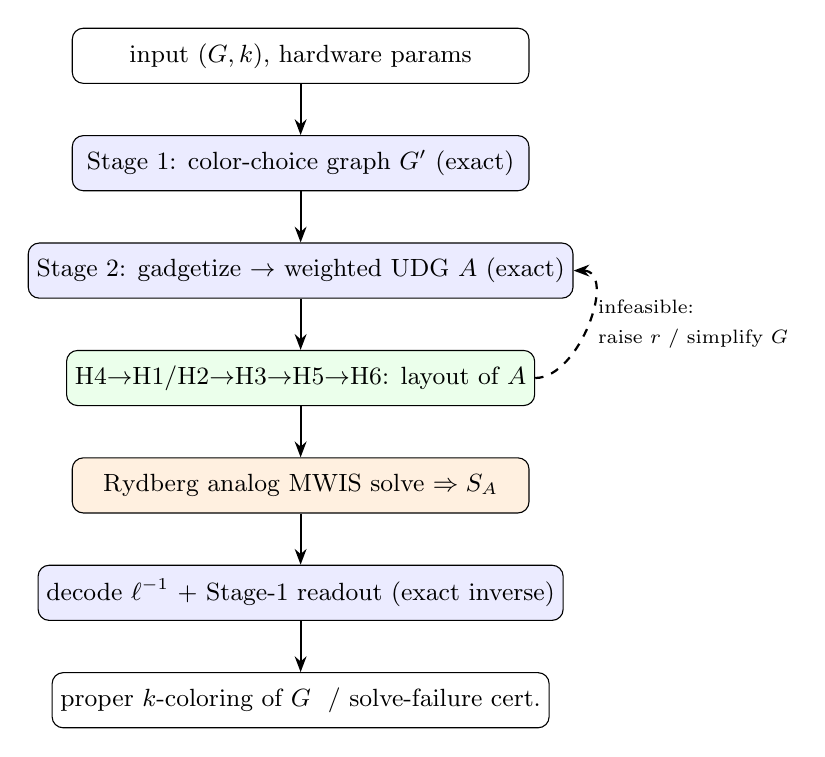
\begin{tikzpicture}[
  font=\small,node distance=6.5mm,
  s/.style={rectangle,draw,rounded corners,minimum width=58mm,minimum height=7mm,align=center,inner sep=3pt},
  ex/.style={s,fill=blue!8}, he/.style={s,fill=green!8}, hw/.style={s,fill=orange!12},
  ar/.style={-{Stealth[length=2mm]},thick}
]
\node[s] (in) {input $(G,k)$, hardware params};
\node[ex,below=of in] (s1) {Stage 1: color-choice graph $G'$ (exact)};
\node[ex,below=of s1] (s2) {Stage 2: gadgetize $\to$ weighted UDG $A$ (exact)};
\node[he,below=of s2] (lay) {H4$\to$H1/H2$\to$H3$\to$H5$\to$H6: layout of $A$};
\node[hw,below=of lay] (solve) {Rydberg analog MWIS solve $\Rightarrow S_A$};
\node[ex,below=of solve] (dec) {decode $\ell^{-1}$ + Stage-1 readout (exact inverse)};
\node[s,below=of dec] (out) {proper $k$-coloring of $G$ \ /\ solve-failure cert.};
\draw[ar](in)--(s1); \draw[ar](s1)--(s2); \draw[ar](s2)--(lay);
\draw[ar](lay)--(solve); \draw[ar](solve)--(dec); \draw[ar](dec)--(out);
\draw[ar,dashed] (lay.east) to[out=0,in=0] node[right,align=left]{\scriptsize infeasible:\\\scriptsize raise $r$ / simplify $G$} (s2.east);
\end{tikzpicture}
\caption{Data flow of Algorithm~\ref{alg:pipeline}. Blue = exact, green = heuristic
layout, orange = analog hardware. Only feasibility, never correctness, flows back.}
\label{fig:flow}
\end{figure}

% =============================================================================
\section{Complexity Analysis}
\label{sec:complexity}
% =============================================================================

Let $N=|V(A)|=O((nk)^2)$ be the atom count. Table~\ref{tab:complexity} summarizes the
per-stage cost. Every stage is polynomial; the exact path is low-degree polynomial, and
the dominant cost is the layout optimization over $N$ atoms.

\begin{table}[h]
\centering
\begin{tabular}{@{}llll@{}}
\toprule
Stage & Cost & Type & Notes \\
\midrule
Stage 1 (color$\to$IS) & $O(nk+mk)$ & exact & build $G'$ \\
Stage 2 (gadgetize)    & $\mathrm{poly}(nk)$, $N=O((nk)^2)$ & exact & Thm.~\ref{thm:gadget} \\
H4 Laplacian init      & $O(N^2)$ (one-time) & heuristic & sparse: $O(Nt)$ \\
H1/H2 optimization     & $O(T\,N^2)$ & heuristic & $T=\mathrm{poly}(N)$ budget \\
H3 clique control      & $O(N\Delta^2)$ per pass & heuristic & local \\
H5 local repair        & $\le \Phi_0$ steps, $\Phi_0=O(N^2\max w)$ & heuristic & $\Phi$-gated, terminates \\
H6 radius sweep        & $O(N^2\log N)$ & heuristic & + $O(N^2)$/radius \\
Decode                 & $O(N)$ & exact & $\ell^{-1}$ + readout \\
\bottomrule
\end{tabular}
\caption{Per-stage complexity. The NP-hardness of UDG \emph{recognition}
\cite{Breu1998} is never incurred: we never decide whether $G$ is a UDG, only realize a
prescribed gadget adjacency.}
\label{tab:complexity}
\end{table}

\begin{proposition}[Polynomial compilation]
With a fixed iteration budget $T=\mathrm{poly}(N)$, Algorithm~\ref{alg:pipeline} runs in
time polynomial in $n$ and $k$ for everything except the analog solve, and emits a
hardware instance of $O((nk)^2)$ atoms together with an exact decoder.
\end{proposition}

\begin{proof}
Sum the rows of Table~\ref{tab:complexity}; each is polynomial in $N=O((nk)^2)$ and
$T=\mathrm{poly}(N)$. Exactness of the emitted decoder is Theorem~\ref{thm:endtoend}.
\end{proof}

% =============================================================================
\section{A Language for Certified Coloring Compilation}
\label{sec:language}
% =============================================================================

Having fixed the semantics, we now give the surface language a programmer writes. It is
\emph{Haskell-flavored} --- pure, statically typed, with algebraic data types,
top-level type signatures written with \texttt{::}, layout-sensitive record syntax, and
pipeline composition --- but it is \emph{not} a general-purpose language. The
differences are deliberate and serve certification.

\subsection{What we keep from Haskell, and what we change}
\label{sec:langdesign}

\begin{table}[h]
\centering
\renewcommand{\arraystretch}{1.2}
\begin{tabular}{@{}p{0.30\linewidth}p{0.62\linewidth}@{}}
\toprule
Haskell-like (kept) & Domain-specific (changed) \\
\midrule
ADTs, records, \texttt{type} synonyms & The base ``values'' are \emph{problems} (graphs,
palettes, instances), not arbitrary data. \\
Top-level signatures \texttt{name :: T} & Types include \emph{problem-types}
$\Col,\ISt,\WIS,\tUDG,\Dev$ (Section~\ref{sec:types}) indexed by size, offset, radius,
spacing. \\
Purity, referential transparency & Total: \textbf{no general recursion}; every program
denotes a finite pipeline that provably terminates. \\
Function arrow \texttt{->} & A second arrow \texttt{\~{}>}, the \emph{certified-reduction}
arrow, is a first-class type former carrying a decoder and an \emph{effect}. \\
Type classes / constraints & A \emph{guarantee lattice} and a \emph{safety effect}
$\{\safe,\asafe{c}\}$ replace ad-hoc constraints; subtyping lets a stronger certificate
stand in for a weaker one. \\
\texttt{>>>}-style composition & Composition threads decoders in reverse and sums
effects; ill-ordered pipelines simply do not type. \\
\bottomrule
\end{tabular}
\caption{Design summary: a small total DSL whose type system is the static shadow of the
reduction theorems.}
\label{tab:langdesign}
\end{table}

\subsection{Concrete grammar}
\label{sec:grammar}

The surface syntax is given below in EBNF. A program is a sequence of typed top-level
bindings; the domain forms (\texttt{graph}, \texttt{palette}, \texttt{restrictions},
\texttt{transform}, \texttt{instance}, \texttt{compute}) are ordinary bindings whose
right-hand side is a domain expression.

\begin{lstlisting}[style=lang]
Program     ::= { Binding }

Binding     ::= [ Signature ] Definition
Signature   ::= Ident "::" Type
Definition  ::= Ident "=" Expr
              | "graph"        Ident "=" GraphExpr
              | "palette"      Ident "=" PaletteExpr
              | "restrictions" Ident "=" "{" { Restriction ";" } "}"
              | "transform"    Ident "=" TransformExpr
              | "instance"     Ident "=" InstanceExpr
              | "compute"      Ident "=" QueryExpr

-- Types: ordinary arrows, problem-types, and the certified-reduction arrow ~>
Type        ::= AType { "->" AType }                 -- ordinary functions
              | Problem "~>" Problem [ "!" Effect ]  -- certified reduction (+ effect)
AType       ::= Problem | "Graph" | "Palette" | "Result" | "(" Type ")"
Problem     ::= "Coloring" Nat Nat                   -- Col<n,k>
              | "IS" Nat                             -- IS<N>
              | "WIS" Nat Nat                        -- WIS<N,C>
              | "UDG" Nat Real Real                  -- UDG<N,r,d>
              | "Dev" Nat                            -- device-feasible
Effect      ::= "safe" | "asafe" Nat

GraphExpr   ::= "graph" "{" "vertices" "=" "[" VertexList "]" ","
                            "edges"    "=" "[" EdgeList "]" "}"
              | "udg" "{" "radius" "=" Real "," "edges" "=" "[" EdgeList "]" "}"
              | "apply" TransformRef "to" GraphRef

PaletteExpr ::= "colors" "[" ColorList "]" | "size" Nat

TransformExpr ::= "toUDG" "(" TransformMode { "," TransformOption } ")"
              | "encodeColoring" Nat                 -- exact gadget encoding
              | "superUDG"                           -- same-vertex supergraph
              | "colorChoice" Nat | "gadgetize" | "layout" Ident | "emit"
              | TransformExpr ">>>" TransformExpr    -- pipeline composition
              | "compose" "[" TransformRefList "]"

TransformMode   ::= "exact" | "preserve" Property
TransformOption ::= "radius" "=" Real | "keep" "=" "[" VertexList "]"
                  | "drop" "=" "[" VertexList "]" | "trackOrigin" "=" Bool
Property        ::= "kColorable" Nat | "chromatic" | "bipartite"

InstanceExpr ::= "color" GraphRef [ "using" PaletteRef ]
                 [ "subjectTo" RestrRef ] [ "via" TransformRef ]
QueryExpr    ::= "chromaticNumber" "(" GraphRef ")"

Restriction  ::= "precolor" Vertex ":" Color
              | "allow" Vertex ":" "[" ColorList "]"
              | "forbid" Vertex ":" "[" ColorList "]"
              | "sameColor" "(" Vertex "," Vertex ")"
              | "differentColor" "(" Vertex "," Vertex ")"
              | "useAtMost" Nat | "useExactly" Nat | "distinctOn" "[" VertexList "]"

Edge       ::= "(" Vertex "," Vertex ")"
Vertex     ::= Ident | Nat        Color ::= Ident | String
Ident      ::= letter { letter | digit | "_" }
Nat        ::= digit { digit }    Real ::= Nat [ "." Nat ]   Bool ::= "true"|"false"
\end{lstlisting}

\subsection{Abstract syntax (Haskell)}
\label{sec:ast}

The AST is itself written in Haskell, emphasizing the family resemblance. Note the
\texttt{Ty} type carries a certified-reduction arrow indexed by source and target
\emph{problem-types} together with an \texttt{Effect}.

\begin{lstlisting}[style=plain]
type Name = String ; type Vertex = String ; type Color = String
type Edge = (Vertex, Vertex) ; type Radius = Double

data Program = Program [Binding]
data Binding = Binding (Maybe Sig) Definition
data Sig     = Sig Name Ty

data Definition
  = DLet          Name Expr
  | DGraph        Name GraphExpr
  | DPalette      Name PaletteExpr
  | DRestrictions Name [Restriction]
  | DTransform    Name TransformExpr
  | DInstance     Name InstanceExpr
  | DQuery        Name QueryExpr

-- Problem-types (the kinds the certified-reduction arrow connects)
data Problem
  = Coloring Int Int          -- Col<n,k>
  | IS Int                    -- IS<N>
  | WIS Int Int               -- WIS<N,C>
  | UDG Int Double Double     -- UDG<N,r,d>
  | Dev Int                   -- device-feasible

data Ty
  = TFun Ty Ty                       -- ordinary  a -> b
  | TReduce Problem Problem Effect   -- certified reduction  A ~> B ! e
  | TGraph | TPalette | TResult

data Effect = Safe | ASafe Int

data TransformExpr
  = ToUDG TransformMode [TransformOption]
  | EncodeColoring Int        -- exact gadget encoding
  | SuperUDG                  -- same-vertex supergraph (carries a safety effect)
  | ColorChoice Int | Gadgetize | Layout Name | Emit
  | Pipe TransformExpr TransformExpr      -- f >>> g
  | Compose [Name]

data TransformMode = Exact | Preserve Property
data Property      = KColorable Int | Chromatic | Bipartite
data TransformOption
  = RadiusOpt Double | KeepVertices [Vertex] | DropVertices [Vertex]
  | TrackOrigin Bool

data GraphExpr   = GraphLit [Vertex] [Edge] | UdgLit Radius [Edge]
                 | ApplyTransform Name Name
data PaletteExpr = ExplicitPalette [Color] | PaletteSize Int
data Restriction = Precolor Vertex Color | Allow Vertex [Color]
                 | Forbid Vertex [Color] | SameColor Vertex Vertex
                 | DifferentColor Vertex Vertex | UseAtMost Int
                 | UseExactly Int | DistinctOn [Vertex]
data InstanceExpr = InstanceExpr
  { instGraph :: Name, instPalette :: Maybe Name
  , instRestrictions :: Maybe Name, instTransform :: Maybe Name }
data QueryExpr = ChromaticNumber Name
\end{lstlisting}

\subsection{Example program}
\label{sec:langexample}

The following program compiles a $3$-coloring of a small graph through the exact gadget
pipeline, and separately exercises the (typed, weaker) supergraph path. The type
signatures are checked by the discipline of Section~\ref{sec:types}.

\begin{lstlisting}[style=lang]
-- input graph and palette ---------------------------------------------------
gInput :: Graph
gInput = graph { vertices = [1,2,3,4,5]
               , edges    = [(1,2),(2,3),(3,1),(1,4),(3,5)] }

pNamed :: Palette
pNamed = colors [red, blue, green]

restrictions rMain = { precolor 1 : red;
                       differentColor (1,2);
                       useAtMost 3 }

-- the exact primary pipeline, fully typed as a chain of certified reductions
encode3 :: Coloring 5 3 ~> Dev 225
encode3 = colorChoice 3 >>> gadgetize >>> layout opts >>> emit

-- run it: the measured bitstring decodes to a proper coloring (soundness)
solve3 :: Result
solve3 = color gInput using pNamed subjectTo rMain via encode3

-- secondary (supergraph) path: SAME vertices, carries a safety effect.
-- Only well-typed when sigma(G) <= 5 ; here it elaborates to `! asafe 1`.
super :: Coloring 5 3 ~> Coloring 5 4 ! asafe 1
super = superUDG

-- a pure query
chiInput :: Int
chiInput = chromaticNumber (gInput)
\end{lstlisting}

% =============================================================================
\section{The Type System}
\label{sec:types}
% =============================================================================

This section gives the type discipline that makes the pipeline's correctness static. It
targets \emph{one thing}: the faithfulness of the compilation \emph{stages}. Ordinary
programming errors --- scope, arity, base types, totality of plain functions --- are
delegated to a standard Hindley--Milner core with refinements; we write
$\Gamma\vdash e:T$ for that judgment and never re-derive it. What we add is a small
\emph{certified-reduction calculus} on top.

\idearemark{The slogan, inherited from type-and-effect
systems~\cite{LucassenGifford1988,BartolettiDeganoFerrariZunino2009}: \emph{base types
say a program is well-formed; problem-types and effects say a \textbf{reduction} is
faithful.} We build only the second.}

\subsection{Problem-types (the sorts)}
\label{sec:sorts}

A \emph{problem-type} names a class of decision/optimization instances together with the
indices we must track to state preservation.

\begin{align*}
A,B \;::=\;
&\ \Col\langle n,k\rangle                       && \text{$k$-coloring instance, $n=|V|$}\\
&\ \Col\langle n,k \mid \beta{:}\,B\rangle       && \text{boundary-precolored ($\beta$ proper on $B\subseteq V$)}\\
&\ \ISt\langle N\rangle\{\,P\,\}                 && \text{independent-set instance, $N$ nodes, refinement $P$}\\
&\ \WIS\langle N,\,C\rangle                       && \text{weighted IS, $N$ nodes, additive offset $C$}\\
&\ \tUDG\langle N,\,r,\,d\rangle                  && \text{\emph{exactly} realized unit-disk inst.\ (radius $r$, spacing $d$)}\\
&\ \tUDGa\langle N,\,r,\,d \mid f\rangle          && \text{\emph{approximately} realized, $f$ residual false edges}\\
&\ \Dev\langle N\rangle \quad (N\le \Nmax)        && \text{device-feasible instance}
\end{align*}

Each $A$ comes with a \emph{solution domain} $\Sol(A)$ and an \emph{optimum}
$\mathrm{opt}(A)\in\mathbb{R}\cup\{\bot\}$. The refinement $P$ on $\ISt$ is where
Stage-1 exactness lives; the canonical one is
\[
  P_{\mathrm{s1}} \;\equiv\; \bigl(\indep = n \iff G \text{ is } k\text{-colorable}\bigr)\ \wedge\ \indep \le n .
\]

\begin{remark}[Why $\tUDGa$ exists]
$\tUDG$ is the placement in which the realized unit-disk graph equals the
\emph{prescribed} gadget adjacency \emph{exactly}. When the layout optimizer leaves
false edges, the object is honestly a \emph{different} graph, so it gets a different
type, $\tUDGa$, and --- crucially --- \textbf{$\tUDGa$ is not a legal source for the
exact decoder} (Section~\ref{sec:stages}). The type is what stops us from silently
reading an answer off a corrupted layout.
\end{remark}

\subsection{The certified-reduction judgment}
\label{sec:judgment}

\begin{definition}[Decoder; total on optima]
A \emph{decoder} from $B$ to $A$ is a partial map
$\delta:\Sol(B)\rightharpoonup\Sol(A)$. It is \emph{total on optima}, written
$\totopt(\delta)$, if $\delta$ is defined on every $s\in\Sol(B)$ with value
$\mathrm{opt}(B)$ and maps it to a value-$\mathrm{opt}(A)$ solution of $A$.
\end{definition}

\begin{definition}[Certified reduction]
The judgment $\vdash\ \tau \;:\; A \;\redto{\delta}\; B$ asserts that $\tau$ takes an
instance of $A$ to an instance of $B$, that $\delta$ is a decoder $B\!\rightharpoonup\!A$
with $\totopt(\delta)$, and that $\mathrm{opt}(A)$ is recoverable as $\delta(s^\star)$
for any optimum $s^\star$ of $B$. Equivalently: \emph{solve $B$ on the device, apply
$\delta$, get the answer to $A$.} This is the surface arrow \texttt{A \~{}> B} of
Section~\ref{sec:language}.
\end{definition}

\subsection{Per-stage typing rules}
\label{sec:stages}

The premises above each line are the proof obligations; in the implementation they are
discharged either by a once-and-for-all proof or by a brute-force oracle on small
instances (Section~\ref{sec:code}).

\paragraph{Stage 1 --- color-choice.}
\[
  \irule{n=|V(G)| \qquad k\ge 1}
        {\vdash\ \mathsf{colorChoice}_k \;:\; \Col\langle n,k\rangle
          \;\redto{\mathsf{decodeColoring}}\; \ISt\langle nk\rangle\{P_{\mathrm{s1}}\}}
  \qquad\rn{S1}
\]
$\mathsf{decodeColoring}$ is total on size-$n$ independent sets and partial elsewhere ---
exactly $\totopt$.

\paragraph{Stage 2 --- gadget.}
\[
  \irule{C = 2\,|E(G')|}
        {\vdash\ \mathsf{gadgetize} \;:\; \ISt\langle N\rangle\{P\}
          \;\redto{\mathsf{decodeLogical}}\; \WIS\langle N+2|E(G')|,\ C\rangle}
  \qquad\rn{S2}
\]
The offset $C$ is carried in the type so ``subtract $C$'' is type-directed;
$\mathsf{decodeLogical}$ (keep logical atoms) is $\totopt$.

\paragraph{Stage 3 --- layout (branches on realizability).} Write $\realizes(p,r)$ for
``the unit-disk graph of $(p,r)$ has edge set exactly $E_A$'' and $\falsep(p,r)$ for the
residual false edges.
\[
  \irule{\realizes(p,r) \qquad \mathsf{spacing}(p)\ge d}
        {\vdash\ \mathsf{layout}(p,r)\;:\; \WIS\langle N,C\rangle
          \;\redto{\mathrm{id}}\; \tUDG\langle N,r,d\rangle}
  \qquad\rn{S3-exact}
\]
\[
  \irule{\miss(p,r)=\varnothing \qquad f=|\falsep(p,r)|>0}
        {\vdash\ \mathsf{layout}(p,r)\;:\; \WIS\langle N,C\rangle
          \;\rightsquigarrow\; \tUDGa\langle N,r,d \mid f\rangle}
  \qquad\rn{S3-approx}
\]
\rn{S3-exact} carries the identity decoder (geometry never relabels a solution) and lands
in $\tUDG$; \rn{S3-approx} carries \emph{no} certified decoder and lands in $\tUDGa$. The
only way to turn $\tUDGa$ back into a legal $\tUDG$ is the metric repair transform that
re-routes false edges through copy/crossing gadgets,
\[
  \irule{\ }
        {\vdash\ \mathsf{nguyen}\;:\; \tUDGa\langle N,r,d\mid f\rangle
          \;\redto{\mathsf{decodeRoute}}\; \WIS\langle N',C'\rangle}
  \qquad\rn{Repair}
\]
after which \rn{S3-exact} can be attempted again.

\paragraph{Emit --- device budget.}
\[
  \irule{N\le \Nmax}
        {\vdash\ \mathsf{emit}\;:\; \tUDG\langle N,r,d\rangle \;\redto{\mathrm{id}}\; \Dev\langle N\rangle}
  \qquad\rn{Fit}
\]

\idearemark{The pipeline can reach $\Dev$ \textbf{only through $\tUDG$}, never through
$\tUDGa$. So ``the machine measured a bitstring'' is connected to ``a correct coloring''
by a \emph{chain of $\totopt$ decoders} --- or it is not connected at all, and the type
checker says so.}

\subsection{Composition and the soundness theorem}
\label{sec:compose}

\[
  \irule{\vdash\ \tau_1 : A \redto{\delta_1} B \qquad \vdash\ \tau_2 : B \redto{\delta_2} C}
        {\vdash\ \tau_2\circ\tau_1 \;:\; A \;\redto{\delta_1\circ\delta_2}\; C}
  \qquad\rn{Comp}
\]

\begin{theorem}[Pipeline soundness]
\label{thm:sound}
If $\vdash\ \Pi \;:\; \Col\langle n,k\rangle \;\redto{\delta}\; \Dev\langle N\rangle$ is
derivable (so $N\le\Nmax$ and every layer is realized \emph{exactly}), then for any
device measurement $m$ with value $\mathrm{opt}(\Dev\langle N\rangle)$, the decoded
$\delta(m)$ is a proper $k$-coloring of $G$ if one exists, and otherwise the pipeline
reports ``not $k$-colorable'' soundly.
\end{theorem}

\begin{proof}[Proof sketch]
By induction on the derivation using \rn{Comp}: each arrow is answer-preserving with a
$\totopt$ decoder, and the composite of $\totopt$ decoders is $\totopt$, so
$\delta=\delta_{\mathrm{s1}}\circ\delta_{\mathrm{s2}}\circ\mathrm{id}\circ\mathrm{id}$
maps an optimum bitstring back through $\WIS$ (strip offset $C$), $\ISt$ (read one slot
per vertex), to a coloring; the refinement $P_{\mathrm{s1}}$ supplies the iff. The only
non-identity geometric step is admitted by \rn{S3-exact}, whose premise $\realizes(p,r)$
guarantees the realized graph \emph{is} $A$, so its optima coincide.
\end{proof}

\begin{corollary}[Ill-ordered pipelines are ill-typed]
\label{cor:order}
Matching the error catalogue (pipeline-stage ordering):
\begin{itemize}[leftmargin=1.4em,itemsep=1pt]
  \item $\mathsf{gadgetize}$ before $\mathsf{colorChoice}$: \rn{S2} expects $\ISt$, is
        given $\Col$ --- no rule applies.
  \item $\mathsf{emit}$ before $\mathsf{layout}$: \rn{Fit} expects $\tUDG$, is given
        $\WIS$.
  \item reading an answer off a false-edged layout: there is no $\totopt$ decoder out of
        $\tUDGa$ (only \rn{Repair}, which goes \emph{back} to $\WIS$).
\end{itemize}
\end{corollary}

\subsection{Refinement A: certificate grade}
\label{sec:grade}

We expose the witness-relative vs.\ true-$\chi$ distinction as a \emph{grade}
$g\in\{\mathsf{w},\chi\}$ on coloring conclusions, with $\mathsf{w}\sqsubseteq\chi$:
$\Col\langle n,k\rangle^{\mathsf{w}}$ is \emph{witness-relative} (a carried coloring
$\kappa$ certifies $\chi(G)\le|\kappa|$ in poly time --- the default), while $\Col\langle
n,k\rangle^{\chi}$ is \emph{exact} ($\chi(G)=k$ as a discharged proof obligation). All
stage rules are grade-polymorphic and preserve the grade; only an explicit
$\mathsf{prove}_\chi$ step (a discharged lower-bound proof, e.g.\ a clique) lifts
$\mathsf{w}\Rightarrow\chi$. Theorem~\ref{thm:sound} holds at grade $\mathsf{w}$ already:
\emph{soundness of compilation does not require knowing the true chromatic number.}

\subsection{Refinement B: the safety effect (supergraph path)}
\label{sec:safety}

The secondary (supergraph) path rewrites $G$ on the \emph{same} vertices by adding edges,
decoded by restriction. Such a transform may inflate $\chi$, so it carries a \emph{safety
effect} $s$ --- a genuine type-and-effect in the sense
of~\cite{BartolettiDeganoFerrariZunino2009}:
\[
  \vdash\ t \;:\; \Col\langle n,k\rangle \;\redtos{\mathsf{restrict}}{s}\; \Col\langle n,k'\rangle,
  \qquad s\in\{\,\safe,\ \asafe{c}\,\}.
\]
$\safe$ means $\chi$ is preserved; $\asafe{c}$ means $t$ never lowers $\chi$ and
$\chi(\text{target})\le\chi(\text{source})+c$.

\paragraph{Effect monoid.}
\[
  \safe\oplus\safe=\safe,\qquad
  \safe\oplus\asafe{c}=\asafe{c},\qquad
  \asafe{c}\oplus\asafe{c'}=\asafe{c+c'}.
\]
Composition combines decoders \emph{and} effects:
\[
  \irule{\vdash t_1 : A \redtos{\delta_1}{s_1} B \qquad \vdash t_2 : B \redtos{\delta_2}{s_2} C}
        {\vdash t_2\circ t_1 : A \redtos{\delta_1\circ\delta_2}{\,s_1\oplus s_2\,} C}
  \qquad\rn{Comp-S}
\]

\paragraph{Mandatory precondition (the impossibility theorem as a side-condition).} A
$\safe$/$\asafe{c}$ introduction is \emph{only} derivable under the neighborhood bound
$\sigma(G)=\max_v\indep(G[N(v)])\le 5$; otherwise the only available type is
$\textsf{unsafe}$ (no $\chi$ certificate). This is exactly the $\chi(K_{1,n})=2$ vs.\
$\chi(H)\ge\lceil n/5\rceil$ obstruction of Theorem~\ref{thm:impossibility}, refusing to
type.

\begin{remark}[Does transform order affect safety?]
Because $\oplus$ sums the bumps $c$ but the \emph{carrier graph} differs between orders,
two orderings of the same multiset of $\asafe{\cdot}$ transforms are type-equal only if
their accumulated bounds \emph{and} side-conditions both match. The type therefore
\emph{records} order-sensitivity as a difference in the derived effect --- turning the
project's open question into a checkable property rather than a conjecture. Correctness,
by contrast, composes order-independently because each arrow is answer-preserving
(Theorem~\ref{thm:sound}); only \emph{cost} and the safety bound are order-sensitive.
\end{remark}

\subsection{The discipline is the static shadow of the oracle}
\label{sec:code}

Every rule corresponds to a function in (or planned for) the Haskell validation harness,
and every premise to a property a brute-force oracle checks; the type system promotes
those runtime checks to static obligations. The recommended minimal core to mechanize
first is \rn{S1}, \rn{S2}, \rn{Comp}, and Theorem~\ref{thm:sound}: the smallest closed
fragment that already makes ``the measured bitstring decodes to a correct coloring'' a
\emph{typed} guarantee.

% =============================================================================
\section{Discussion and Limitations}
\label{sec:discussion}
% =============================================================================

\paragraph{What is and isn't guaranteed.} The reduction is exact and verifiable: a
decoded set of size $n$ is a certified coloring. What is \emph{not} guaranteed is that
the analog device reaches the MWIS ground state, or that a large instance fits the array.
These are physics and capacity questions, cleanly separated from correctness by
Theorem~\ref{thm:endtoend} and from typing by Theorem~\ref{thm:sound}.

\paragraph{The size wall.} The $O((nk)^2)$ atom budget is the binding constraint against
present devices of a few hundred atoms~\cite{Wurtz2023}; in the worst case this admits
only a handful of original vertices. We treat this as an honest limitation, not the
headline: the value of the framework --- the exact reduction, the impossibility result,
the type-and-effect discipline --- is independent of $N_{\max}$ and durable as hardware
scales. The leverage against the wall is preprocessing (graph simplification, crossing
minimization, decomposition) and the layout optimizer; quantifying the achievable
reduction on structured instances is the main empirical question this design opens.

\paragraph{Status of the secondary path.} The stand-alone supergraph backend is retained
only for theory and comparison. By Theorem~\ref{thm:impossibility} it is unbounded on
general graphs, and it additionally requires iterated independent-set extraction to color
on hardware. Its practically valuable contribution is its geometric machinery, which the
primary path reuses as the layout optimizer.

% =============================================================================
\section{Future Work}
\label{sec:future}
% =============================================================================

Two engineering forks remain open: \emph{which gadget set} to adopt (the verbatim
construction of~\cite{Nguyen2023} versus a custom set, affecting what must be re-proved),
and confirming the \emph{weighted} MWIS interface end-to-end. On the language side, the
next steps are to mechanize the minimal core (Section~\ref{sec:code}) in a proof
assistant or as liquid refinements, to add the decomposition layer (precolor / split /
stitch with a typed device budget $(wk)^2\le\Nmax$), and to wire the type checker to the
validation harness so that absent proofs fall back to the oracle on small instances.
Empirically, we plan an evaluation in Bloqade against QuEra-class
parameters~\cite{Wurtz2023}, measuring atom count, area, crossing number, and
ground-state success probability across structured and random instances.

% =============================================================================
\section{Conclusion}
\label{sec:conclusion}
% =============================================================================

Neutral-atom hardware solves UDG--MWIS, not coloring, and that single fact selects the
architecture. Compiling coloring exactly means \emph{reducing} it to UDG--MWIS via the
classical colorability$\to$independent-set reduction composed with Rydberg copy/crossing
gadgetization --- a once-proved, inflation-free, polynomial pipeline with an exact
decoder. The geometric heuristics that a supergraph approach would have leaned on for
correctness are provably unable to bound chromatic inflation on general graphs; their
proper and sound home is the layout optimizer that fits the exact gadget instance onto
the device. On top of this semantic substrate sits a small Haskell-flavored language
whose type-and-effect discipline makes provenance, stage ordering, the device budget, and
chromatic safety static, so that a well-typed program is a certified compiler. This
separation --- exact correctness in the reduction, heuristic effort in the geometry,
behavioral guarantees in the types --- is the foundation we offer, and the connection to
type-and-effect systems is one we are glad to dedicate to Gian-Luigi Ferrari.

% =============================================================================
\bibliographystyle{plain}
\bibliography{references}
% =============================================================================

\end{document}
